\section{Processos de Software}

Engenharia de Software pode ser definida como:
\begin{citacao}[english]
1. the systematic application of scientific and technological knowledge, methods, and experience to the design,
implementation, testing, and documentation of software [...]  2. the application
of a systematic, disciplined, quantifiable approach to the development, operation,
and maintenance of software; that is, the application of engineering to software \cite{IEEE2010}.
\end{citacao}

A engenharia de software deve ter foco na qualidade, que apoia as outras camadas
dessa tecnologia, que são as camadas de processo, métodos e ferramentas \autoref{fig:desen_engsoft}.
A camada de processo define um conjunto de atividades ou um arcabouço que tem
como finalidade garantir a efetiva utilização da tecnologia engenharia de software, que dessa forma
leva à produção de um software. Os detalhes de como fazer o software pertencem
a camada de métodos. Os métodos da engenharia de software incluem tarefas de planejamento
e estimativa de software, análise de requisitos, modelagem de projeto, codificação,
testes e manutenção. As ferramentas de engenharia de software auxiliam as camadas de
processo e métodos, com ferramentas automatizadas, que por sua vez, quando integradas,
é estabelecido um suporte ao desenvolvimento de software chamado CASE -
\textit{Computer Aided Software Engineering} \cite{Pressman2009, Sommerville2006}.

\begin{figure}[b]
  \centering
  \caption{Engenharia de Software - uma tecnologia em camadas}
  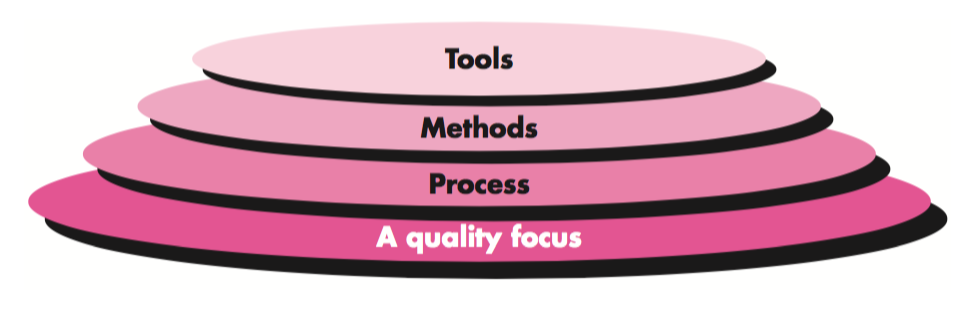
\includegraphics[scale=0.3]{imagens/desenv_engsoft2}
  \label{fig:desen_engsoft}
  \fonte{\cite{Pressman2009}}
\end{figure}

Entre o conjunto de atividades definidas pela camada de processo, quatro são
fundamentais, a saber, especificação de software, projeto e implementação de
software, validação de software e evolução de software. Especificação de software
ou engenharia de requisitos é uma fase importante e crítica do processo de engenharia
de software. Importante porque é uma análise de requisitos bem feita que possibilitará
atendar as demandas dos usuários. Crítica porque um sistema mal especificado, pode até ser
bem projetado e construído, mas não vai atender as necessidades dos usuários.
Em seguida, na fase de projeto e implementação os requisitos são projetados e programados,
tendo como resultado um sistema executável. Depois, o software deve ser verificado
para mostrar que atende às demandas dos usuários (validação do software). Finalmente,
na fase de evolução de software, o mesmo é modificado devido às mudanças
de requisitos e às necessidades dos usuários.

Quanto ao modelos de engenharia de software temos os modelos prescritivos e os ágeis.
Os modelos prescritivos definem um conjunto de atividades explícitas para serem
desenvolvidos no processo de engenharia de software. O Processo Unificado de desenvolvimento
tem o maior destaque e reconhencimento dentre os modelos prescritivos.

\subsection{Processo Unificado}
O Processo Unificado define quatro atividades no processo de desenvolvimento de software.
As fases são descritas como:

\begin{description}
  \item [{Concepção:}] Por meio da comunicação com os clientes, um conjunto
  preliminar de casos de uso UML e da arquitetura do sistema é elaborada.
  \item [{Elaboração:}] Nessa fase, os casos de uso UML são expandidos e
  refinados, bem como a definição da arquitetura do sistema. Ao final
  dessa fase, um conjunto de casos de uso UML descrevem os requisitos
  dos sistema. Uma descrição da arquitetura do sistema e um plano de
  desenvolvimento do software também são esperados.
  \item [{Construção:}] Os casos de uso UML desenvolvidos na fase de elaboração
  são então desenvolvidos e testados. O software deve estar funcionando
  e documentado na conclusão dessa fase.
  \item [{Transição:}] transferência do software aos usuários finais.
\end{description}

Fluxos de trabalhos ou \emph{workflows} ocorrem durante todas as
fases no processo de desenvolvimento. São seis \emph{workflows} principais
e três de apoio:
\begin{enumerate}
  \item \emph{Modelagem de negócios}: processos de negócios modelados por
  casos de uso.
  \item \emph{Requisitos}: atores são idenficados e casos de uso são desenvolvidos.
  \item \emph{Análise e projeto: }vários modelos são desenvolvidos como de
  arquitetura e componentes.
  \item \emph{Implementação: }componentes são implementados.
  \item \emph{Teste: }processo iterativo em conjunto com a implementação.
  \item \emph{Implantação: }software é distribuído aos usuários finais.
  \item \emph{Gerenciamento de configuração e mudança: }apoio as mudanças
  do sistema.
  \item \emph{Gerenciamento de projeto: }apoio de desenvolvimento do sistema.
  \item \emph{Meio ambiente: }apoio a equipe de desenvolvimento com ferramentas.
\end{enumerate}

\subsection{Métodos Ágeis}

Contrapondo-se aos modelos prescritivos em que propoem especificar por completo
os requisitos do sistema e só então projetar, construir e testar o sistema, surgiu
os métodos ágeis, que têm como filosofia o manifesto ágil. Esse manifesto afirma:

\begin{citacao}
  Estamos descrobrindo melhores maneiras de desenvolver softwares, fazendo-o e ajudando
  outros a fazê-lo. Através dessse trabalho, valorizamos mais:\\\\
  \begin{minipage}{15cm}
    \begin{itemize}
      \item Indivíduos e interações do que processos e ferramentas
      \item Software em funcionamento do que documentação abrangente
      \item Colaboração do cliente do que negociação de contrato
      \item Resposta a mudanças do que seguir um plano
    \end{itemize}
  \end{minipage}\\\\
  Ou seja, embora itens à direita sejam importantes, valorizamos mais os que estão à esquerda.
\end{citacao}

Abordagens ágeis incluem Extreme Programming e o Scrum. Eles propõem diferentes processos
para que tenha-se um desenvolvimento e entrega incremental do sistema, tendo em comum princípios
baseados no manifesto ágil.


\section{Metodologias e Ferramentas}
A metodologia escolhida nesse projeto levou em consideração as necessidades de um trabalho de
conclusão de curso no curto prazo e os recursos limitados. Adicionalmente, a falta de uma documentação
mínima (como documentação de requisitos, diagramas de classes, atores e componentes do sistema)
pode ser uma barreira para a entrada de contribuidores para projetos de software livre. Dessa forma,
uma abordagem baseada em metodologias ágeis para modelagem, documentação codificação.

\subsection{Objetivos específicos}

Para cada objetivo específico deste trabalho, as seguintes técnicas e ferramentas foram utilizadas:

\subsubsection{Realizar levantamento de requisitos sobre os sistemas de resposta em sala de aula}

O processo de elicitação de requisitos do sistema utilizou a análise de competidores que
consistiu basicamente em buscar em alguns sistemas de resposta existentes, referências positivas e
negativas para definição do modelo a ser proposto.

\subsubsection{Especificar e implementar uma aplicação para dispositivos móveis, que será utilizado como {\clickers}}

Com os requistos da primeira etapa, tivemos os requisitos inicias para a aplicação móvel.
A linguagem de programação usada na fase de implementação do aplicativo foi JavaScript, tendo como auxílio o framework Ionic.

O Ionic é um framework de código aberto para o desenvolvimento de aplicativos híbridos e desktop utilizando
tecnologias web como HTML, CSS e JavaScript otimizados para dispositivos móveis, com código fonte sobre a licença MIT.

\subsubsection{Especificar e implementar uma aplicação web para o professor administrar as questões e gerar relatórios}

Com os requistos da primeira etapa, tivemos os requisitos inicias para a aplicação desktop do professor.
O Ionic também foi utilizado na aplicação desktop do professor.

\subsubsection{Especificar e implementar um sistema servidor, para receber e
    enviar dados para os os clientes: dispositivos móveis dos alunos e navegador
    web do professor}

O sistema servidor foi desenvolvido utilizando tecnologias como Node.js, Express, MongoDB, Socket.io e Feathers.
Tais tecnlogias foram utilizadas por permitir o fácil desenvolvimento de aplicações
de tempo real entre o servidor e os seus clientes.

A teoria mais aprofundada sobre os métodos e ferramentas citadas serão descritas nas próximas seções.

\section{Requisitos do Sistema}

\subsection{Análise de competidores}

A análise de competidores é uma técnica oriunda engenharia da usabilidade
que consiste em avaliar produtos concorrentes em busca de pontos positivos e
negativos. Tal técnica é útil no levantamento de requisitos de um novo sistema,
identificação de pontos fortes e fracos os produtos, reutilização de design, dentre outros.

Avaliar produtos concorrentes é valioso, porque oferece a oportunidade de novos
produtos evitarem problemas existentes dos competidores, explorar os pontos
fracos, além da reutilização dos pontos positivos.

A análise de competidores foi utilizada neste trabalho para elicitar requisitos e boas práticas
de design de interfaces. % bem como evitar problemos já identificados pelos concorrentes
Os resultados obtidos foram utilizados no processo de definição do
protótipo de alta fidelidade.

\subsubsection{Socrative}

Socrative é um sistema de resposta específico para usar em salas de aula. O sistema pode ser
acessado pelo site ou nos aplicativos para iOS e Android. No socrative, apenas o professor
precisa fazer um cadastro no site (questões demográficas são solicitadas). Existe uma versão
gratuita e paga do aplicativo.

Na conta do professor, é possível criar questionários de múltipla escolha, verdadeira e falso e
de questões abertas. Quando o professor cria uma conta, é gerado um código de identificação
para que os alunos possam entrar na sala virtual. Na interface do estudante, é necessário
colocar o código de identificação do professor.

\subsubsection{PollEverywhere}

O PollEverywhere é um sistema de resposta mais genérico, possibilitando fazer votações em
shows e apresentações diversas. Possibilita integração com ferramentas de apresentação
como o PowerPoint. Outra característica é a possibilidade dos usuários votarem por SMS.
Além dos tipos de questões básicas, o PollEverywhere permite criar nuvem de palavras e
questões com imagens clicáveis.

A conta do usuário é associado com uma URL, em que é usada para os participantes
da votação entrarem e votarem.

\subsubsection{TopHat}

TopHat é outra solução voltada para a educação, contando com seis tipos de questões.
Adicionalmente o TopHat permite ao professor fazer a chamada dos estudantes, isso porque
o professor pode gerar um código aleatório no TopHat para que os estudantes presentes
possam enviar o código e marcar presença. O produto também disponibiliza uma sala
de discussão e a possibilidade de criar slides dentro do aplicativo.

\begin{center}
\begin{table}
\begin{centering}
\begin{tabular}{>{\centering}m{4cm}||>{\centering}p{4cm}>{\centering}p{3.5cm}c}
\hline
\multicolumn{1}{>{\centering}m{3.5cm}}{Caraterística} & PollEverywhere & TopHat & Socrative\tabularnewline
\hline
\hline
Open-Source & Não & Não & Não\tabularnewline
Integração com LMS & Blackboard & Excel & MasteryConnect\tabularnewline
Formatos & JSON, RSS, CSV & Não & Não\tabularnewline
Read-only API & Sim & Não & Não\tabularnewline
Integração com PowerPoint & Possibilita & Não & Não\tabularnewline
Métodos de votação & SMS, web & SMS, Web & Internet\tabularnewline
Tempo-real & Sim & Sim & Sim\tabularnewline
Acesso ao sistema & URL & Código de Acesso & Código de Acesso\tabularnewline
Tipos de questões & 5 & 7 & 3\tabularnewline
Mínimo de passos para votação & 2 & 3 & 4\tabularnewline
Anonimato & Possibilita & Possibilita & Possibilita\tabularnewline
Contagem regressiva & Possibilita & Possibilita & Não\tabularnewline
Download CSV & Possibilita & Não & Não\tabularnewline
Relatórios por estudante & Possibilita & Possibilita & Não\tabularnewline
\hline
\end{tabular}
\par\end{centering}

\caption{Análise de Competidores}
\end{table}

\par\end{center}

\subsection{Requisitos gerados a partir da análise de competidores}

A partir das informações coletadas na análise de competidores, foram
extraídos um conjunto de requisitos iniciais para o sistema. Os requisitos gerados
pela análise dos competidores foram os seguintes:

\begin{description}
\item[Integração com sistemas LMS]: O sistema deve permitir integração com
sistemas LMS (preferencialmente Moodle);
\item[Todas as plataformas:] é muito importante que o sistema seja capaz
de funcionar em smartphones, tables e computadores independentemente
do sistema operacional.
\item[Questões abertas, verdadeiro/falso e de múltipla-escolha:] O sistema
deve fornecer pelo menos esses três tipos básico de questões;
\item[Modo de votação:] O sistema deve permitir votação anonima ou requisitar
a identificação;
\item[Customização das questões:] O sistema deve permitir inserção de equações
matemáticas (\LaTeX), imagens e texto como opção das questões;
\item[Controle da votação:] Opções básicas como ativar ou desativar a votação
e limpar uma votação em andamento;
\item[Controle de frequência:] o sistema gera um código aleatório ou uma
questão trivial, em que o professor pode solicitar que os estudantes
respondam, contando como controle de frequência. Os dados devem ser
facilmente exportados para CSV.
\item[Tempo-real:] No momento da votação, o professor pode escolher entre
apresentar o resultado em tempo-real, quando todos votarem, ou quando
determinado;
\item[Banco de questões:] As questões elaboradas pelo professor podem ser
armazenadas em um banco de questões que o sistema deve manter;
\item[Facilidade do uso e de criação de votação:] O sistema não deve oferecer
dificuldades de uso e de criação de questões;
\item[Código de acesso:] O sistema deve gerar um código de acesso único para
identificar o ambiente do professor, usado para que os alunos respondam.
\end{description}








\subsection{Prototipação}

A prototipação trouxe benefícios ao trabalho na medida em que instrumentalizou várias
funcionalidades do sistema de avaliação e permitiu também, embora de maneira
preliminar, verificar alguns aspectos de usabilidade, provocando, por exemplo, alguns
reposicionamentos dos componentes da tela de modo a torná-los mais evidentes para os
usuários.
